\documentclass[12pt]{article}
\usepackage[dvipsnames]{xcolor}
\usepackage{hyperref, pagecolor, mdframed }
\usepackage{graphicx, amsmath, latexsym, amsfonts, amssymb, amsthm,
amscd, geometry, xspace, enumerate, mathtools}
\usepackage{tikz}

\theoremstyle{plain}
\newtheorem{thm}[subsubsection]{Th\'eor\`eme}
\newtheorem{lem}[subsubsection]{Lemme}
\newtheorem{rem}{Remarque}

\theoremstyle{definition}
\newtheorem{defn}[subsubsection]{D\'efinition}

\theoremstyle{remark}


\hypersetup{
    colorlinks=true,
    linkcolor=blue,
    urlcolor=Green,
    filecolor=RoyalPurple
}

\definecolor{wgrey}{RGB}{148, 38, 55}


\title{Protocoles réseaux : sécurité}
\date{30 octobre 2023}
\begin{document}
\maketitle
\begin{enumerate}
    \item Politiques de sécurité (ce que/qui je veux empecher de faire quoi)
    \item Modèle d'attaque (ce que l'attaquant a le droit de faire)
\end{enumerate}

\noindent \textbf{Propriétés de sécurité} qui définissent les politiques de securité :
\begin{enumerate}
    \item confidentialité \begin{enumerate}
        \item anonymat/"méta-données"
        \item 
    \end{enumerate}
    \item authenticité
    \item integrité
    \item disponibilité, absence de déni. (par ex : un serveur doit être accessible)
\end{enumerate}

\noindent \textbf{Types d'authentifications}:
\begin{enumerate}
    \item chiffrage ad hoc, clé négociée, pas d'auth (pb de man in the middle)
    \item TOFU "trust on first use", leap of faith
    \item authentification certifiée (mac)
\end{enumerate}

\section{SSL/TLS et https}
HTTP: pas de mécanisme de sécurité $\rightarrow$ \begin{itemize}
    \item SSL$\rightarrow$ auth, chiffrage
\end{itemize}

HTTPS: HTTP+auth(du serveur)+confidentialité.

\section{Pas de couche de convergence}
Avant : Seulement IP, en vrai : couche 2/3/4, 802.2/IP/TCP/TLS/HTTP. 

Si on choisit http comme couche de convergence :
\begin{itemize}
    \item Beaucoup d'overhead (headers ?)
    \item pas de temps reel
    \item pas de pair à pair
\end{itemize}

\noindent Temps réel $<50ms$:
\begin{itemize}
    \item audio $\subseteq$ vidéoconférence
    \item jeux en ligne
    \item broadcasting (foot)
    \item VR\\
\end{itemize}

\noindent Triangle de Chrobozsceck(massacre):\begin{center}

\indent \indent 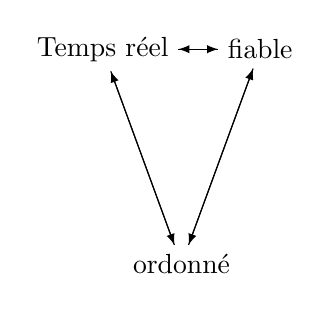
\begin{tikzpicture}[x=1cm,y=1cm,>=latex,->]
    \node(0) at (-90:1) {ordonné};
    \node(1) at (60 : 2) {fiable};
    \node(2) at (120 : 2) {Temps réel};

    \foreach \k/\l in {0/1, 0/2, 1/2, 2/1, 1/0, 2/0}{\draw(\k)--(\l);}
\end{tikzpicture}
\end{center}

\begin{rem}
    Autres protocoles: \begin{enumerate}
        \item SCTP \begin{enumerate}
            \item $\rightarrow$ sémantique par messages
            \item $\rightarrow$ partiellement ordonné: flots multiples
            \item $\rightarrow$ fiable/non-fiable
        \end{enumerate}
        \item DCCP$\rightarrow$ jamais vu
    \end{enumerate}
Problème :\begin{itemize}
    \item ne traverse pas les NAT
    \item sécurité ?
\end{itemize}
\end{rem}

\newpage
Solution:
\subsection{Protocoles basés sur UDP}
On met UDP entre IP et transport et pour éviter que Le
NAT regarde dans les paquets : On chiffre avant la couche transport. On obtient
\begin{enumerate}
    \item IP$\rightarrow$UDP$\rightarrow$DTLS(Datagram TLS)$\rightarrow$transport.
\end{enumerate}

\noindent On peut maintenant utiliser:\\
\indent $\rightarrow$ SCTP over DTLS(pas à la mode).\\
\indent $\rightarrow$ QUICK\begin{itemize}
            \item $\rightarrow$intégré avec TLS! (le handshake se fait en un seul RTT au lieu de deux)
            \item $\rightarrow$Probleme, c'est a nouveau une sémantique par flots d'octets multiples(y'a aussi par message)
            (obligé d'avoir un buffer+pb de perte de paquets en plein milieu)(possible de faire plusieurs choses en meme temps)
            \item par message $\rightarrow$ non fiable/non ordonné, par flots $\rightarrow$ fiable, ordonné
\end{itemize}

Pas possible de faire du pair à pair: TLS! Les téléphones/particuliers ont des NAT, pas de certificats, juste une adresse ip.\\
\indent $\rightarrow$ Solution: UDP brut.
Plusieurs pbs: \begin{enumerate}
    \item Problème du rendez-vous(général), comment on contacte qqun en UDP?
    \item Problème de la traversée du NAT.
    \item crypto: auth.
\end{enumerate}
Trop difficile. A la place : \textbf{UDP+contrôle}, on ajoute un serveur qui controle
\begin{itemize}
    \item Les rendez-vous(vie privée)
    \item Echanges cryptographique (voir tp7)
    \item Traversée de NAT (voir projet)
\end{itemize}

BitTorrent: Le fichier telechargé contient un hash qui permet l'authentification au serveur, pb, toutes les ips sont traquées.













\end{document}